\documentclass[border=8pt]{standalone}
\usepackage{tikz}
\usetikzlibrary{arrows.meta}
\usepackage{amsmath}

\definecolor{evidence}{HTML}{2196F3}
\definecolor{choice}{HTML}{E91E63}
\definecolor{causal}{HTML}{FF9800}
\definecolor{neutral}{HTML}{9E9E9E}

\begin{document}
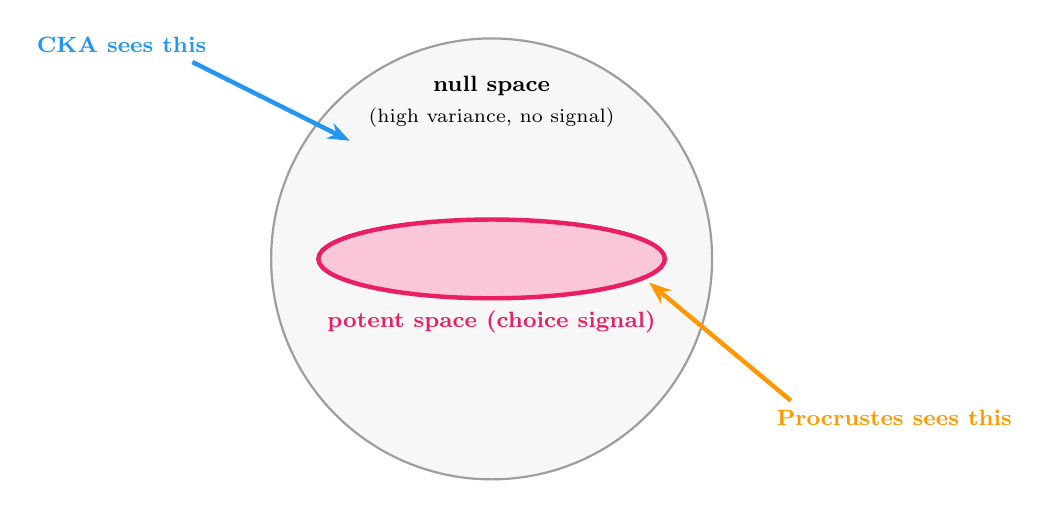
\begin{tikzpicture}

  % Null space (big circle)
  \fill[neutral!8] (3,3) ellipse (2.8 and 2.8);
  \draw[neutral,thick] (3,3) ellipse (2.8 and 2.8);
  \node[black,font=\footnotesize\bfseries,align=center] at (3,5.2) {null space};
  \node[black,font=\scriptsize,align=center] at (3,4.8) {(high variance, no signal)};

  % Potent space (thin horizontal ellipse inside)
  \fill[choice!25] (3,3) ellipse (2.2 and 0.5);
  \draw[choice,ultra thick] (3,3) ellipse (2.2 and 0.5);
  \node[choice,font=\footnotesize\bfseries] at (3,2.2) {potent space (choice signal)};

  % CKA arrow — pointing at outer circle
  \draw[evidence,ultra thick,-{Stealth[length=8pt]}] (-0.8,5.5) -- (1.2,4.5);
  \node[evidence,font=\footnotesize\bfseries,anchor=south east] at (-0.5,5.5) {CKA sees this};

  % Procrustes arrow — pointing at inner ellipse
  \draw[causal,ultra thick,-{Stealth[length=8pt]}] (6.8,1.2) -- (5,2.7);
  \node[causal,font=\footnotesize\bfseries,anchor=north west] at (6.5,1.2) {Procrustes sees this};

\end{tikzpicture}
\end{document}
